%%% Document Author: J Moss
%%% Parts in LaTeX: Nicholas Dart
%%% Other Content: See authors list
%%% Document Last edit: 28.10.2014

\documentclass[11pt, article]{article}
\usepackage{a4wide}
\usepackage[english]{babel}
\usepackage{graphicx}
\usepackage{tabu}
\usepackage{textcomp}
\usepackage{fancyhdr}
\usepackage{lastpage}
\usepackage{titlesec}
\usepackage{lscape}
\usepackage{longtable}
\usepackage{color}
\usepackage{listings}

\definecolor{mygreen}{rgb}{0,0.6,0}
\definecolor{mygray}{rgb}{0.5,0.5,0.5}
\definecolor{mymauve}{rgb}{0.58,0,0.82}

\lstset{ % Syntax highliughting for java
    backgroundcolor=\color{white},   % choose the background color; you must add \usepackage{color} or \usepackage{xcolor}
    basicstyle=\footnotesize,        % the size of the fonts that are used for the code
    breakatwhitespace=false,         % sets if automatic breaks should only happen at whitespace
    breaklines=true,                 % sets automatic line breaking
    captionpos=b,                    % sets the caption-position to bottom
    commentstyle=\color{mygreen},    % comment style
    deletekeywords={...},            % if you want to delete keywords from the given language
    escapeinside={\%*}{*)},          % if you want to add LaTeX within your code
    extendedchars=true,              % lets you use non-ASCII characters; for 8-bits encodings only, does not work with UTF-8
    frame=none,                    % adds a frame around the code
    keepspaces=true,                 % keeps spaces in text, useful for keeping indentation of code (possibly needs columns=flexible)
    keywordstyle=\color{blue},       % keyword style
    language=Octave,                 % the language of the code
    morekeywords={*,...},            % if you want to add more keywords to the set
    numbers=left,                    % where to put the line-numbers; possible values are (none, left, right)
    numbersep=5pt,                   % how far the line-numbers are from the code
    numberstyle=\tiny\color{mygray}, % the style that is used for the line-numbers
    rulecolor=\color{black},         % if not set, the frame-color may be changed on line-breaks within not-black text (e.g. comments (green here))
    showspaces=false,                % show spaces everywhere adding particular underscores; it overrides 'showstringspaces'
    showstringspaces=false,          % underline spaces within strings only
    showtabs=false,                  % show tabs within strings adding particular underscores
    stepnumber=5,                    % the step between two line-numbers. If it's 1, each line will be numbered
    stringstyle=\color{mymauve},     % string literal style
    tabsize=4,                       % sets default tabsize to 2 spaces
    title=\lstname                   % show the filename of files included with \lstinputlisting; also try caption instead of title
}

%%%%%%
%% Variables for version and release status
%% useage: \version
%%%%%%
\newcommand\version{0.3}
\newcommand\release{Pre-Release}
\newcommand\titleText{Design Specification}
\newcommand\reference{SE\_NO2\_MAN\_01}

%%%%%%
%% Alias
%%%%%%
\newcommand{\sectionbreak}{\clearpage}  %% Allways start a section on a new page

\title{ \huge CS221 Group Project \\ \Large \titleText}
\author{
    \vspace{100pt}
    \begin{tabular}{ r || l }
        Project Team    & jcm14, acb12, mta2, wia3, \\
                        & nid21, msh4, jao14, mip34, \\
                        & set12, daw54, anw46 \\
                        & \\
        Version         & \version \\
        Status          & \release \\
        Date Published  & \today \\
        Reference       & \reference \\
        Department      & Computer Science \\
        Address         & Aberystwyth University \\
                        & Penglais Campas \\
                        & Ceredigion \\
                        & SY23 3DB \\
    \end{tabular} \\
    Copyright \textcopyright Aberystwyth University 2014
    %get rid of the date on the titlepage
    \date{}
}

\pagestyle{fancy}
\fancyhf{}
\rhead{Version \version (\release)}
\rfoot{Page \thepage \hspace{1pt} of \pageref{LastPage}}
\lfoot{Aberystwyth University - Computer Science}

\begin{document}
    \setcounter{page}{1}

    \maketitle

    \tableofcontents

    \section{Decomposition Description}
        \subsection{Subsystems}
	The Botanist Tools application is composed of 3 subsystems:
	\begin{itemize}
		\item Android Application
		\item Website
		\item Server
	\end{itemize}

	\subsubsection{Android Application}
		The android application provides the interface that users will use to record  plant data when out on a visit. It implements requirements (FR1), (FR2), (FR3), (FR4), (FR5), (FR6). It must also conform with the requirements (EIR1), (PR1),  (PR2), (DC1) and (DC2)~\cite{refSpec}.

		The application will have a form-based activity which can be used to add and edit new and currently saved recordings. Currently saved recordings will be stored locally in a collection, which will be awaiting dispatch to the server. The user will be able to view this list and select recordings to perform actions on (Eg. edit and delete). The application will not show recordings that are saved on the server. 

		The Android application will communicate with the server to perform functions such as sending recordings and performing user authentication. The application does NOT communicate directly with the website and the database. It uses a web API which is core to the server.

	\subsubsection{Server}

		The server will consist of two parts: 
		\begin{itemize}
			\item A database
			\item A web API
		\end{itemize}

	\subsubsection{Database}
		The database will be the central datastore for the entire system. It will communicate exclusively with the web API and serve as its back-end. 

	\subsubsection{Web API}
		The web API is central to the system; it provides a uniform way of accessing the database for all subsystems to use. It maintains the integrity of the datastore by acting as the ``middle-man'' so that the other subsystems do not damage the contents. It exposes a public interface to allow a set of actions to be performed by the users of the API; actions include user authentication and recordings management. The web API will implement the requirement (FR7) and must also conform to the requirement (PR2).

	\subsubsection{Website}
		The website will consist of a set of web-pages which implement all the required functionalities for the user (FR8) and (FR9). It must also conform to the requirements (EIR1), (PR1) and (PR2). The website will communicate with the Web API via HTTP to receive from and send data to the database. The website will have no communication with the Android application. It will also not directly communicate with the database, but will go through the web API. 


\subsection{Significant Android Components}

	\subsubsection{Significant UI classes}
		\begin{tabular}{r p{10cm}}
		HomeActivity & This class will hold the code to allow a user to move on to the NewRecordingActivity via a startNewRecordingButton. \\

		NewRecordingActivity & This class will hold the code to allow a user to enter information such as Name, Phone Number, E-Mail, and Site Location. It will also allow the application to receive date and time information from the Android device. The nextButton will then move the user to the AddNewSpeciesActivty. \\

		AddNewSpeciesActivity & This class will hold the code to allow a user to enter all the required information about a species entry in the current recording. It allows you to choose the name of a species from a locally saved list, and also allows the user to add a new species name, if not found. This activity must have the functionality to use the device's GPS capabilities to record location information of the species. It allows the user to select abundance in accordance with the DAFOR scale. The user should be able to add a scene/specimen picture through the device's camera or the gallery application. The user can also add a note if they wish. There is then a confirmButton which adds the species to the current recording and moves the user on to the MaintainRecordingActivity. \\

		MaintainRecordingActivity & This class will hold the code to allow a user to maintain the current recording. It will contain the functionality to edit any entered species from the collection in the recording. It will also allow the user to delete the current recording, removing all stored species data. The user will be able to save the recording, sending the current recording to the server at the first opportunity. \\
		\end{tabular}

	\subsection{Significant other classes}
		\begin{tabular}{r p{13cm}}
		Specimen & This class will hold the code to define all the information a specimen object can hold. Fields to hold this data will be: speciesName, gpsLocation, abundance, scenePicture, specimenPicture, notes. This class will also provide getter and setter methods for the mentioned fields.\\

		Recording & This class will hold the code to define all the information a recording object will hold. Fields to hold this data will be: usersName, usersPhoneNumber, usersEmail, usersAddress, dateTime. This class will contain getters and setters for the mentioned fields.\\
		\end{tabular}

\subsection{Significant Website Components}
	\begin{tabular}{r p{10cm}}
	Navigation & A set of buttons at the top of each webpage that will allow the user to move around the site. When clicking on the desired button, they will be taken to the designated page.\\

	Homepage & This landing page will provide all the general information a user needs to know about the service. It also contains a search bar which will allow the user to filter through the plant database to find what they are looking for. \\

	View Species Page & This page will display every species in the database for the user to view and select. If the user selects a species, they will be taken to the View Chosen Species Page, which provides more species information. This page will also allow the user to add a new species, taking them to the Add Species Page. \\

	View Chosen Species Page & This page will display all information about the specific species chosen by the user. \\

	Add Species Page & This page will provide all the forms necessary to input all data for a chosen species (name, location, abundance, scene picture, specimen pictures and notes), or allow a user to add a new species that is not listed. \\

	Map Overlay & This component will be a pop-up map that will show the locations of the chosen species. This location will be taken from the database.\\
	\end{tabular}

\clearpage
\subsection{Significant Server Components}

	\begin{tabular}{r p{10cm}}
	Server & A database and a set of Web API commands to allow manipulation. \\
	Database & a MySQL database where we will store all data for our system \\
		\begin{itemize}
			\item Tables 
			\begin{itemize}
				\item botany_users
				\item botany_records
				\item botany_specimens
				\item botany_reserves
				\item botany_resources
			\end{itemize}
		\end{itemize}
	Web API & A list of commands that allow the Android and website systems to access and manipulate data in the Database. \\
		\begin{itemize}
			\item addRecord.php - Adds a record to the database
			\item addReserve.php - Adds a reserve to the database
			\item addResource.php - Adds a resource (picture) to the database
			\item  authenticateAdmin.php - Checks an inputted password and tells if it's the same as the stored password
			\item getRecord.php - Returns a record 
			\item getRecords.php - Returns all records
			\item getReserve.php - Returns a reserve
			\item getReserves.php - Returns all reserves
			\item getResource.php - Returns a resource (picture)
			\item getSpecimen.php - Returns a specimen
			\item getSpecimens.php - Returns all specimens
			\item removeReserve.php - Removes a reserve
			\item removeSpecimen.php - Removes a specimen
			\item updateReserve.php - Updates a reserve
			\item updateSpecimen.php - Updates a specimen
		\end{itemize}

    \section{Android Application Design}
        \subsection{Decompisition}
	The compilation dependencies are as follows:
	\begin{itemize}
		\item Android dependencies a user will have an array of visits
		\item A visit will have an array of specimens
		\item A specimen can get data from the plant db (Fig \ref{fig:androidComponentDiagram}).
	\end{itemize}
	
	\begin{figure}
		\centering
			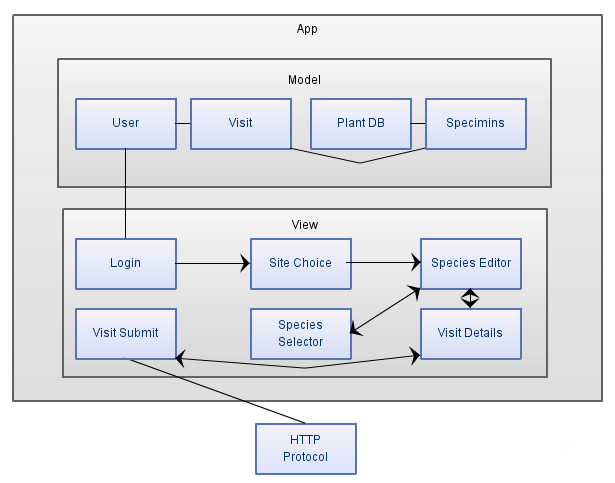
\includegraphics[scale=0.75]{android/componentDiagram.png}
		\caption{Component diagram for Android}
		\label{fig:androidComponentDiagram}
	\end{figure}

\newpage
\subsection{Interfaces}
	\subsubsection{Login Activity Interface}
		\lstinputlisting[language=Java, firstline=33]{android/src/loginInterface.java}

	\newpage
	\subsubsection{Site Choice Activity Interface}
		\lstinputlisting[language=Java, firstline=8]{android/src/siteChoiceInterface.java}

	\newpage
	\subsubsection{Species Selector Activity Interface}
		\lstinputlisting[language=Java, firstline=8]{android/src/speciesSelectorInterface.java}

	\newpage
	\subsubsection{Visit Management Activity Interface}
		\lstinputlisting[language=Java, firstline=8]{android/src/visitManagementInterface.java}

	\newpage
	\subsubsection{Visit Submit Activity Interface}
		\lstinputlisting[language=Java, firstline=8]{android/src/visitSubmitInterface.java}

	\newpage
	\subsubsection{User Data Class Interface}
		\lstinputlisting[language=Java, firstline=1]{android/src/userClassInterface.java}

	\subsubsection{Visit Data Class Interface}
		\lstinputlisting[language=Java, firstline=1]{android/src/visitClassInterface.java}

	\subsubsection{Plant DB Interface}
		This Will be a file obtained from the Botanical Society of Britain and Ireland containing a large list of known plant types in a comma sperated list (CSV) format. This file will be parsed at runtime and a condensed list created in alphabetical order for searching. Obtained from $http://www.bsbi.org.uk/resources.html$

	\subsubsection{Specimen Class Interface}
		\lstinputlisting[language=Java, firstline=1]{android/src/SpecimenClassInterface.java}


    %%\begin{landscape}

        %%\section{Bar}
            %%\input{far/foo.tex}

    %%\end{landscape}

    \section{Document History}
        \begin{tabular}{l || p{10cm} | l | r}
            Version & Edit & Date & Persons \\ \hline 
            0.1 & Initial Version & November 5 2014 & nid21 \\ \hline
            0.2 & Updated with decomposition description & November 12 2014 & nid21 \\
            0.3 & Updated with Android interfaces & November 17 2014 & nid21 \\
        \end{tabular}

\end{document}